%----------------------------------------------------------------------------------------
%	PACKAGES AND THEMES
%----------------------------------------------------------------------------------------

\documentclass{beamer}
\usepackage{ragged2e}
\justifying

\mode<presentation> {
\usetheme{CambridgeUS}
%\usetheme{AnnArbor}
\usecolortheme{dolphin}
%\usecolortheme{crane}
\setbeamertemplate{navigation symbols}{}}

\usepackage{scrextend}
\usepackage[utf8]{inputenc}
\usepackage[]{algorithm2e}
\usepackage[T1]{fontenc}
\usepackage[british]{babel}
\usepackage{amsmath,amsthm,amssymb,amsfonts}
\usepackage{enumerate}
\usepackage{wrapfig}
\newcommand{\bm}{\boldsymbol}
\newcommand{\ds}{\displaystyle}
\newcommand{\mA}{{\mathbb A}}
\newcommand{\mB}{{\mathbb B}}
\newcommand{\mC}{{\mathbb C}}
\newcommand{\mD}{{\mathbb D}}
\newcommand{\mE}{{\mathbb E}}
\newcommand{\mI}{{\mathbb I}}
\newcommand{\mN}{{\mathbb N}}
\newcommand{\mQ}{{\mathbb Q}}
\newcommand{\mP}{{\mathbb P}}
\newcommand{\mR}{{\mathbb R}}
\newcommand{\mS}{{\mathbb S}}
\newcommand{\mZ}{{\mathbb Z}}
\newcommand{\cA}{{\mathcal A}}
\newcommand{\cb}{{\mathcal B}}
\newcommand{\cC}{{\mathcal C}}
\newcommand{\cE}{{\mathcal E}}
\newcommand{\cF}{{\mathcal F}}
\newcommand{\cG}{{\mathcal G}}
\newcommand{\cH}{{\mathcal H}}
\newcommand{\cI}{{\mathcal I}}
\newcommand{\cJ}{{\mathcal J}}
\newcommand{\cL}{{\mathcal L}}
\newcommand{\cM}{{\mathcal M}}
\newcommand{\cO}{{\mathcal O}}
\newcommand{\cP}{{\mathcal P}}
\newcommand{\cT}{{\mathcal T}}
\newcommand{\cU}{{\mathcal U}}
\newcommand{\cV}{{\mathcal V}}
\newcommand{\cZ}{{\mathcal Z}}
\newcommand{\sM}{{\mathscr M}}
\newcommand*{\defeq}{\mathrel{\vcenter{\baselineskip0.5ex \lineskiplimit0pt
                     \hbox{\scriptsize.}\hbox{\scriptsize.}}}%
                     =}
\usepackage{mathrsfs}
\usepackage{framed}
\usepackage{courier}


\theoremstyle{plain}
\newtheorem{thm}{Theorem}[section]
\newtheorem{prop}[thm]{Proposition}
\newtheorem{lem}[thm]{Lemma}
\newtheorem{cor}[thm]{Corollary}
\newtheorem{conj}[thm]{Conjecture}
\newtheorem*{conj*}{Conjecture}

\theoremstyle{definition}
\newtheorem{dfn}{Definition}[section]
\newtheorem{ex}{Example}[section]
\newtheorem{pbm}{Problem}[section]
\newtheorem{opbm}{Open problem}[section]
\newtheorem*{opbm*}{Open problem}

\theoremstyle{remark}
\newtheorem{obs}{Observation}[section]
\newtheorem{nota}{Notation}[section]
\newtheorem{ter}{Terminology}[section]

\usepackage{rotating,tabularx}

\newcommand{\quotes}[1]{``#1''}


%----------------------------------------------------------------------------------------
% GRAPHICS
%----------------------------------------------------------------------------------------

\usepackage{graphicx}
\usepackage{tikz}
\usepackage{epstopdf}
\usepackage{color}
\definecolor{mygreen}{rgb}{0,0.6,0}
\definecolor{myred}{RGB}{139,0,0}
\definecolor{myblue}{RGB}{0,0,205}
\definecolor{myorange}{RGB}{255,140,0}
\usepackage{booktabs} % Allows the use of \toprule, \midrule and \bottomrule in tables

%----------------------------------------------------------------------------------------
%	TITLE PAGE
%----------------------------------------------------------------------------------------

\title[]{Complex Networks}
\author[]{Montserrat Brufau Vidal\\ Àlex Ferrer Campo}
\institute[]{Universitat de Barcelona}
\date{2018}

\AtBeginSection[] % Do nothing for \section*
{
\begin{frame}<beamer>[noframenumbering]
\frametitle{Outline}
\tableofcontents[currentsection]
\end{frame}
}

%\AtBeginSubsection[] % Do nothing for \section*
%{
%\begin{frame}<beamer>[noframenumbering]
%\frametitle{Outline}
%\tableofcontents[currentsection,currentsubsection]
%\end{frame}
%}

\begin{document}

\begin{frame}
\titlepage
\end{frame}

\begin{frame}
\frametitle{Contents}
\tableofcontents
\end{frame}

%----------------------------------------------------------------------------------------
%	PRESENTATION SLIDES
%----------------------------------------------------------------------------------------

\section{Summary of the chosen data}

%------------------------------------------------

\begin{frame}
\frametitle{DNC emails}
\begin{block}{About this network}
	Directed network of \textbf{emails} in the 2016 Democratic National Committee email leak. The Democratic National Committee (DNC) is the formal governing body for the United States Democratic Party. A dump of emails of the DNC was leaked in 2016 by Wikileaks. 
\end{block}
\pause
\begin{itemize}
	\item \textbf{Nodes:} \textbf{People} in the dataset.
	\pause
	\item \textbf{Edges:} A directed edge in the dataset denotes that a person has sent an \textbf{email} to another person. Since an email can have any number of recipients, a single email is mapped to multiple edges in this dataset.
	\pause
	\item \textbf{Extra data:} Every edge has the \textbf{timestamp} indicating the time where the email was sent.
\end{itemize}
\textbf{Source:} \href{https://github.com/renepickhardt/dnc-email-crunching}{https://github.com/renepickhardt/dnc-email-crunching}

\end{frame}

%------------------------------------------------

\begin{frame}
\frametitle{DNC emails}

\begin{figure}
	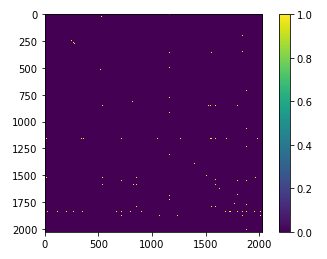
\includegraphics[height=0.75\textheight,keepaspectratio]{figures/ad_mat_snapshot}
	\caption{Adjacency Matrix.}
\end{figure}
\end{frame}

%------------------------------------------------
\section*{}
\begin{frame}

\centering
\Huge{Thank you for your attention!}

\end{frame}

%----------------------------------------------------------------------------------------

\end{document}